\documentclass[11pt,a4paper]{article}

% Packages
\usepackage[utf8]{inputenc}
\usepackage[T1]{fontenc}
\usepackage{lmodern}
\usepackage[margin=1in]{geometry}
\usepackage{graphicx}
\usepackage{tikz}
\usetikzlibrary{shapes,arrows,positioning,fit,backgrounds,calc,decorations.pathreplacing}
\usepackage{listings}
\usepackage{xcolor}
\usepackage{hyperref}
\usepackage{amsmath}
\usepackage{amssymb}
\usepackage{booktabs}
\usepackage{multirow}
\usepackage{float}
\usepackage{fancyhdr}
\usepackage{titlesec}
\usepackage{tcolorbox}
\tcbuselibrary{listings,breakable}

% Code listing style
\definecolor{codebg}{RGB}{248,248,248}
\definecolor{codeframe}{RGB}{200,200,200}
\definecolor{keywordcolor}{RGB}{0,0,180}
\definecolor{commentcolor}{RGB}{0,128,0}
\definecolor{stringcolor}{RGB}{163,21,21}

\lstdefinestyle{rustcode}{
    language=C,
    backgroundcolor=\color{codebg},
    frame=single,
    rulecolor=\color{codeframe},
    basicstyle=\ttfamily\small,
    keywordstyle=\color{keywordcolor}\bfseries,
    commentstyle=\color{commentcolor}\itshape,
    stringstyle=\color{stringcolor},
    numbers=left,
    numberstyle=\tiny\color{gray},
    breaklines=true,
    showstringspaces=false,
    tabsize=4,
    morekeywords={pub,fn,struct,impl,let,mut,async,await,Arc,Self,u64,u8,f64,i64,Option,Result,Vec,HashMap}
}

% Header/Footer
\pagestyle{fancy}
\fancyhf{}
\rhead{BetterBot Systems Architecture}
\lhead{Binance Price Feed}
\rfoot{Page \thepage}

% Title formatting
\titleformat{\section}{\Large\bfseries\color{blue!70!black}}{\thesection}{1em}{}
\titleformat{\subsection}{\large\bfseries\color{blue!50!black}}{\thesubsection}{1em}{}

% Document info
\title{
    \vspace{-1cm}
    \textbf{Binance Price Feed Architecture} \\
    \large Low-Latency Market Data Integration for BetterBot \\
    \vspace{0.5cm}
    \normalsize Technical Reference Document v1.0
}
\author{BetterBot Systems Engineering}
\date{January 2026}

\begin{document}

\maketitle
\thispagestyle{empty}

\begin{abstract}
This document provides a comprehensive technical overview of the Binance price feed integration within BetterBot. It covers the multi-tier architecture designed for high-frequency market data ingestion, including the primary \texttt{barter-data} based feed, the optimized \texttt{BinanceBookTickerFeed} with SIMD-accelerated parsing, the zero-overhead HFT ingest path with SeqLock synchronization, and the hardened production wrapper with session management. Additionally, this document details the latency measurement harness, metrics collection infrastructure, and the edge receiver architecture for ultra-low latency deployments.
\end{abstract}

\tableofcontents
\newpage

%==============================================================================
\section{Executive Summary}
%==============================================================================

The Binance price feed is a critical component of BetterBot's FAST15M trading engine, providing real-time top-of-book data for BTC, ETH, SOL, and XRP pairs. The architecture is designed with multiple layers optimized for different latency-sensitivity requirements:

\begin{itemize}
    \item \textbf{Layer 1}: \texttt{BinancePriceFeed} -- Production-ready feed using \texttt{barter-data} crate with broadcast channel delivery
    \item \textbf{Layer 2}: \texttt{BinanceBookTickerFeed} -- Optimized bookTicker stream with SIMD JSON parsing and ArcSwap snapshots
    \item \textbf{Layer 3}: \texttt{BinanceHftIngest} -- Zero-allocation hot path with SeqLock synchronization and CPU pinning
    \item \textbf{Layer 4}: \texttt{HardenedBinanceIngest} -- Production wrapper with state machine, exponential backoff, and circuit breakers
    \item \textbf{Layer 5}: \texttt{EdgeReceiver} -- UDP multicast edge architecture for sub-millisecond latency (experimental)
\end{itemize}

\begin{tcolorbox}[title=Key Performance Metrics,colback=green!5!white,colframe=green!50!black]
\begin{tabular}{ll}
\textbf{Decode Latency (p99):} & $< 100 \mu s$ \\
\textbf{Internal Processing:} & $< 500 \mu s$ \\
\textbf{Wire Latency (EU $\rightarrow$ Binance):} & $20-50$ ms \\
\textbf{Memory Allocation (hot path):} & Zero \\
\textbf{Reconnect Backoff:} & $100$ ms -- $30$ s (exponential with jitter) \\
\end{tabular}
\end{tcolorbox}

%==============================================================================
\section{System Architecture Overview}
%==============================================================================

\subsection{High-Level Data Flow}

\begin{figure}[H]
\centering
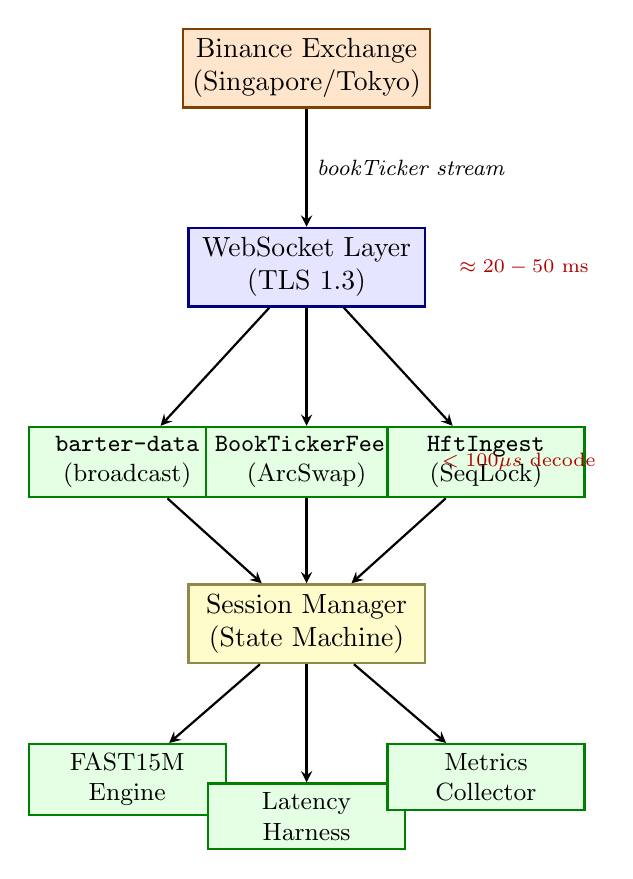
\begin{tikzpicture}[
    node distance=1.5cm,
    box/.style={rectangle, draw=blue!50!black, fill=blue!10, thick, minimum height=1cm, minimum width=3cm, align=center},
    smallbox/.style={rectangle, draw=green!50!black, fill=green!10, thick, minimum height=0.8cm, minimum width=2.5cm, align=center, font=\small},
    arrow/.style={->, thick, >=stealth},
    label/.style={font=\footnotesize\itshape}
]

% Binance
\node[box, fill=orange!20, draw=orange!50!black] (binance) {Binance Exchange\\(Singapore/Tokyo)};

% WebSocket Layer
\node[box, below=of binance] (ws) {WebSocket Layer\\(TLS 1.3)};

% Ingest Options
\node[smallbox, below left=1.5cm and -0.5cm of ws] (barter) {\texttt{barter-data}\\(broadcast)};
\node[smallbox, below=of ws] (bookticker) {\texttt{BookTickerFeed}\\(ArcSwap)};
\node[smallbox, below right=1.5cm and -0.5cm of ws] (hft) {\texttt{HftIngest}\\(SeqLock)};

% Session Management
\node[box, fill=yellow!20, draw=yellow!50!black, below=3.5cm of ws] (session) {Session Manager\\(State Machine)};

% Consumers
\node[smallbox, below left=1cm and -0.5cm of session] (fast15m) {FAST15M\\Engine};
\node[smallbox, below=of session] (latency) {Latency\\Harness};
\node[smallbox, below right=1cm and -0.5cm of session] (metrics) {Metrics\\Collector};

% Arrows
\draw[arrow] (binance) -- node[right, label] {bookTicker stream} (ws);
\draw[arrow] (ws) -- (barter);
\draw[arrow] (ws) -- (bookticker);
\draw[arrow] (ws) -- (hft);
\draw[arrow] (barter) -- (session);
\draw[arrow] (bookticker) -- (session);
\draw[arrow] (hft) -- (session);
\draw[arrow] (session) -- (fast15m);
\draw[arrow] (session) -- (latency);
\draw[arrow] (session) -- (metrics);

% Latency annotations
\node[right=0.3cm of ws, font=\scriptsize, text=red!70!black] {$\approx 20-50$ ms};
\node[right=0.3cm of bookticker, font=\scriptsize, text=red!70!black] {$< 100 \mu s$ decode};

\end{tikzpicture}
\caption{Binance Price Feed Data Flow Architecture}
\label{fig:dataflow}
\end{figure}

\subsection{Component Responsibilities}

\begin{table}[H]
\centering
\begin{tabular}{lp{8cm}}
\toprule
\textbf{Component} & \textbf{Responsibility} \\
\midrule
\texttt{BinancePriceFeed} & Primary feed using \texttt{barter-data}; broadcast channel for reactive consumers; EWMA volatility calculation \\
\texttt{BinanceBookTickerFeed} & Optimized direct WebSocket; SIMD JSON parsing via \texttt{simd-json}; lock-free reads via \texttt{ArcSwap} \\
\texttt{BinanceHftIngest} & Zero-allocation hot path; SeqLock snapshots; CPU pinning; dedicated ingest thread \\
\texttt{HardenedBinanceIngest} & Production wrapper; state machine; exponential backoff with jitter; endpoint rotation; circuit breakers \\
\texttt{SessionManager} & Connection lifecycle; heartbeat monitoring; resync coordination; proactive refresh (23h) \\
\texttt{BinanceLatencyHarness} & Comprehensive latency measurement; histogram statistics; CSV export; Grafana dashboard spec \\
\midrule
\texttt{EdgeReceiver} & UDP multicast from co-located edge node; loss detection; reorder buffer; QUIC fallback \\
\bottomrule
\end{tabular}
\caption{Component Responsibilities}
\end{table}

%==============================================================================
\section{Layer 1: BinancePriceFeed (barter-data)}
%==============================================================================

\subsection{Overview}

The \texttt{BinancePriceFeed} provides a production-ready interface using the \texttt{barter-data} crate. It subscribes to L1 orderbook streams and broadcasts price updates via \texttt{tokio::sync::broadcast}.

\begin{lstlisting}[style=rustcode, caption=BinancePriceFeed Core Structure]
pub struct BinancePriceFeed {
    inner: Arc<RwLock<HashMap<String, SymbolState>>>,
    max_history_len: usize,     // ~3h at 1Hz
    ewma_lambda: f64,           // 0.97
    update_tx: broadcast::Sender<PriceUpdateEvent>,
}
\end{lstlisting}

\subsection{Key Features}

\begin{itemize}
    \item \textbf{Symbols}: BTCUSDT, ETHUSDT, SOLUSDT, XRPUSDT
    \item \textbf{Update Rate}: $\approx 1$ Hz per symbol (L1 orderbook)
    \item \textbf{History Buffer}: 10,800 points (3 hours at 1Hz)
    \item \textbf{Volatility}: EWMA variance with $\lambda = 0.97$
    \item \textbf{Broadcast Capacity}: 1024 events
\end{itemize}

\subsection{Volatility Estimation}

The feed computes per-second log return volatility using exponentially weighted moving average:

\begin{equation}
\sigma^2_t = \lambda \cdot \sigma^2_{t-1} + (1 - \lambda) \cdot r_t^2
\end{equation}

where $r_t = \ln(P_t / P_{t-1}) / \Delta t$ and $\lambda = 0.97$.

%==============================================================================
\section{Layer 2: BinanceBookTickerFeed (Optimized)}
%==============================================================================

\subsection{Design Principles}

The \texttt{BinanceBookTickerFeed} is optimized for minimal latency with the following design principles:

\begin{enumerate}
    \item Direct WebSocket connection to Binance bookTicker stream
    \item SIMD-accelerated JSON parsing (\texttt{simd-json})
    \item Zero heap allocations on hot path
    \item Lock-free reads via \texttt{ArcSwap}
    \item Sequence tracking with gap detection
    \item CPU-pinned receive task
    \item Async metrics collection off hot path
\end{enumerate}

\subsection{Architecture Diagram}

\begin{figure}[H]
\centering
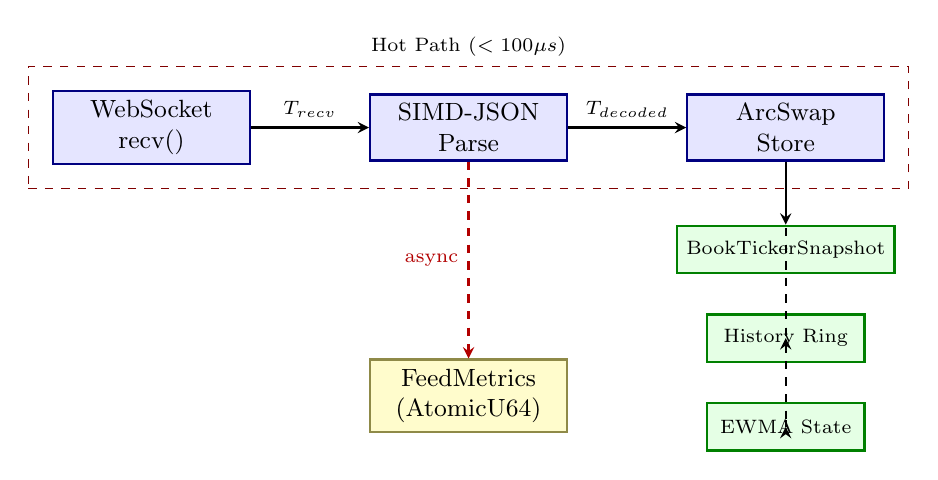
\begin{tikzpicture}[
    node distance=1cm,
    process/.style={rectangle, draw=blue!50!black, fill=blue!10, thick, minimum height=0.8cm, minimum width=2.5cm, align=center, font=\small},
    data/.style={rectangle, draw=green!50!black, fill=green!10, thick, minimum height=0.6cm, minimum width=2cm, align=center, font=\scriptsize},
    arrow/.style={->, thick, >=stealth}
]

% Hot Path
\node[process] (ws) {WebSocket\\recv()};
\node[process, right=1.5cm of ws] (simd) {SIMD-JSON\\Parse};
\node[process, right=1.5cm of simd] (arcswap) {ArcSwap\\Store};

% Data structures
\node[data, below=0.8cm of arcswap] (snapshot) {BookTickerSnapshot};
\node[data, below=0.5cm of snapshot] (history) {History Ring};
\node[data, below=0.5cm of history] (ewma) {EWMA State};

% Metrics (cold path)
\node[process, fill=yellow!20, draw=yellow!50!black, below=2.5cm of simd] (metrics) {FeedMetrics\\(AtomicU64)};

% Arrows
\draw[arrow] (ws) -- node[above, font=\scriptsize] {$T_{recv}$} (simd);
\draw[arrow] (simd) -- node[above, font=\scriptsize] {$T_{decoded}$} (arcswap);
\draw[arrow] (arcswap) -- (snapshot);
\draw[arrow, dashed] (arcswap) |- (history);
\draw[arrow, dashed] (arcswap) |- (ewma);
\draw[arrow, dashed, red!70!black] (simd) -- node[left, font=\scriptsize, text=red!70!black] {async} (metrics);

% Timing box
\node[draw=red!50!black, dashed, fit=(ws)(simd)(arcswap), inner sep=0.3cm, label={[font=\scriptsize]above:Hot Path ($< 100 \mu s$)}] {};

\end{tikzpicture}
\caption{BinanceBookTickerFeed Hot Path Architecture}
\end{figure}

\subsection{BookTickerSnapshot Structure}

\begin{lstlisting}[style=rustcode, caption=Zero-Allocation Snapshot Structure]
#[derive(Debug, Clone, Copy, Default)]
pub struct BookTickerSnapshot {
    pub update_id: u64,
    pub exchange_ts_ms: i64,      // Wall-clock reference only
    pub recv_mono_ns: u64,        // Monotonic recv timestamp
    pub decoded_mono_ns: u64,     // Monotonic decode complete
    pub bid_price: f64,
    pub bid_qty: f64,
    pub ask_price: f64,
    pub ask_qty: f64,
}
\end{lstlisting}

\subsection{SIMD JSON Parsing}

The feed uses \texttt{simd-json} for high-performance parsing:

\begin{lstlisting}[style=rustcode, caption=SIMD-Accelerated JSON Parsing]
fn parse_combined_stream(
    raw: &mut [u8],
    recv_mono_ns: u64,
) -> Result<(Symbol, BookTickerSnapshot), ParseError> {
    let value = simd_json::to_borrowed_value(raw)?;
    let obj = value.as_object().ok_or(ParseError::NotObject)?;
    let data = obj.get("data").ok_or(ParseError::MissingField("data"))?;
    // Extract fields with zero-copy...
}
\end{lstlisting}

\subsection{Metrics Collection}

Metrics are collected atomically off the hot path:

\begin{table}[H]
\centering
\begin{tabular}{lll}
\toprule
\textbf{Metric} & \textbf{Type} & \textbf{Description} \\
\midrule
\texttt{decode\_latency\_*} & AtomicU64 & Sum, count, max of decode latencies \\
\texttt{jitter\_*} & AtomicU64 & Inter-arrival jitter statistics \\
\texttt{messages\_received} & AtomicU64 & Total messages processed \\
\texttt{parse\_errors} & AtomicU64 & JSON parse failures \\
\texttt{gaps\_total} & AtomicU64 & Sequence gaps detected \\
\texttt{reconnects} & AtomicU64 & WebSocket reconnection count \\
\bottomrule
\end{tabular}
\caption{FeedMetrics Atomic Counters}
\end{table}

%==============================================================================
\section{Layer 3: BinanceHftIngest (Zero-Overhead)}
%==============================================================================

\subsection{Design Goals}

\begin{enumerate}
    \item \textbf{Minimize userspace overhead}: No allocations in hot path
    \item \textbf{Deterministic latency}: Pinned thread, preallocated buffers
    \item \textbf{Lock-free reads}: Multiple consumers cannot block each other
    \item \textbf{Last-value semantics}: Slow consumers see latest data, skip intermediate
\end{enumerate}

\subsection{SeqLock Synchronization}

The SeqLock pattern provides lock-free synchronization for single-writer, multiple-reader scenarios:

\begin{figure}[H]
\centering
\begin{tikzpicture}[
    node distance=0.5cm,
    step/.style={rectangle, draw=blue!50!black, fill=blue!10, thick, minimum height=0.6cm, minimum width=4cm, align=center, font=\small}
]

% Writer side
\node[step] (w1) {Increment seq to odd (write start)};
\node[step, below=of w1] (w2) {Memory fence (release)};
\node[step, below=of w2] (w3) {Write tick data};
\node[step, below=of w3] (w4) {Memory fence (release)};
\node[step, below=of w4] (w5) {Increment seq to even (write complete)};

% Reader side
\node[step, right=3cm of w1] (r1) {Load seq1 (acquire)};
\node[step, below=of r1] (r2) {If odd: spin\_loop, retry};
\node[step, below=of r2] (r3) {Read tick data};
\node[step, below=of r3] (r4) {Memory fence (acquire)};
\node[step, below=of r4] (r5) {Load seq2; if seq1 $\neq$ seq2: retry};

% Labels
\node[above=0.3cm of w1, font=\bfseries] {Writer (Single Thread)};
\node[above=0.3cm of r1, font=\bfseries] {Reader (Any Thread)};

\end{tikzpicture}
\caption{SeqLock Protocol for Lock-Free Reads}
\end{figure}

\begin{lstlisting}[style=rustcode, caption=SeqLock Implementation]
#[repr(C, align(64))]
pub struct SeqLockSnapshot {
    seq: AtomicU64,           // Odd = write in progress
    tick: UnsafeCell<PriceTick>,
    _pad: [u8; SEQLOCK_PAD_SIZE],  // Cache line padding
}

impl SeqLockSnapshot {
    #[inline(always)]
    pub fn write(&self, tick: PriceTick) {
        let old = self.seq.load(Relaxed);
        self.seq.store(old + 1, Release);  // Start (odd)
        fence(Release);
        unsafe { *self.tick.get() = tick; }
        fence(Release);
        self.seq.store(old + 2, Release);  // Complete (even)
    }
    
    #[inline(always)]
    pub fn read(&self) -> Option<PriceTick> {
        for _ in 0..10 {
            let seq1 = self.seq.load(Acquire);
            if seq1 & 1 == 1 { spin_loop(); continue; }
            if seq1 == 0 { return None; }
            let tick = unsafe { *self.tick.get() };
            fence(Acquire);
            if seq1 == self.seq.load(Acquire) { return Some(tick); }
            spin_loop();
        }
        None
    }
}
\end{lstlisting}

\subsection{CPU Pinning (Linux)}

For deterministic latency, the ingest thread can be pinned to a dedicated CPU core:

\begin{lstlisting}[style=rustcode, caption=CPU Affinity Setting]
#[cfg(target_os = "linux")]
if let Some(core) = config.pin_to_core {
    unsafe {
        let mut cpuset: libc::cpu_set_t = std::mem::zeroed();
        libc::CPU_SET(core, &mut cpuset);
        libc::sched_setaffinity(0, size_of::<cpu_set_t>(), &cpuset);
    }
}
\end{lstlisting}

\subsection{Performance Comparison}

\begin{table}[H]
\centering
\begin{tabular}{lcc}
\toprule
\textbf{Aspect} & \textbf{broadcast::channel} & \textbf{SeqLock} \\
\midrule
Slow consumer behavior & Creates lag (backpressure) & Sees latest value \\
Memory usage & $O(\text{buffer} \times \text{consumers})$ & $O(1)$ per symbol \\
Allocation in hot path & Per-message clone & Zero \\
Read latency & $\approx 500$ ns (channel ops) & $\approx 50$ ns (atomic load) \\
Missed updates & Error (RecvError::Lagged) & Silent skip (by design) \\
\bottomrule
\end{tabular}
\caption{Broadcast Channel vs SeqLock Comparison}
\end{table}

%==============================================================================
\section{Layer 4: HardenedBinanceIngest (Production)}
%==============================================================================

\subsection{State Machine}

\begin{figure}[H]
\centering
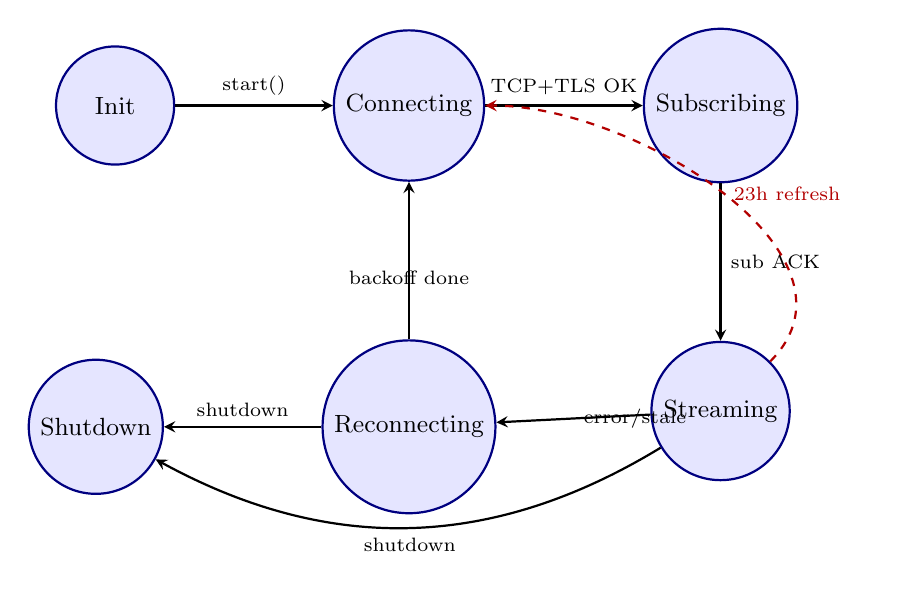
\begin{tikzpicture}[
    state/.style={circle, draw=blue!50!black, fill=blue!10, thick, minimum size=1.5cm, align=center, font=\small},
    arrow/.style={->, thick, >=stealth},
    label/.style={font=\scriptsize, midway}
]

\node[state] (init) {Init};
\node[state, right=2cm of init] (connecting) {Connecting};
\node[state, right=2cm of connecting] (subscribing) {Subscribing};
\node[state, below=2cm of subscribing] (streaming) {Streaming};
\node[state, below=2cm of connecting] (reconnecting) {Reconnecting};
\node[state, left=2cm of reconnecting] (shutdown) {Shutdown};

\draw[arrow] (init) -- node[above, label] {start()} (connecting);
\draw[arrow] (connecting) -- node[above, label] {TCP+TLS OK} (subscribing);
\draw[arrow] (subscribing) -- node[right, label] {sub ACK} (streaming);
\draw[arrow] (streaming) -- node[right, label] {error/stale} (reconnecting);
\draw[arrow] (reconnecting) -- node[below, label] {backoff done} (connecting);
\draw[arrow] (streaming) to[bend left] node[below, label] {shutdown} (shutdown);
\draw[arrow] (reconnecting) -- node[above, label] {shutdown} (shutdown);

% Proactive refresh loop
\draw[arrow, dashed, red!70!black] (streaming) to[out=45, in=0] node[right, label, text=red!70!black] {23h refresh} (connecting);

\end{tikzpicture}
\caption{HardenedBinanceIngest State Machine}
\end{figure}

\subsection{Exponential Backoff with Jitter}

To prevent thundering herd on mass reconnects, backoff uses jitter:

\begin{equation}
\text{backoff}_n = \min\left(\text{base} \times 2^n, \text{max}\right) \times (1 \pm \text{jitter})
\end{equation}

\begin{table}[H]
\centering
\begin{tabular}{lll}
\toprule
\textbf{Parameter} & \textbf{Default} & \textbf{Env Override} \\
\midrule
Base backoff & 100 ms & \texttt{BINANCE\_BACKOFF\_BASE\_MS} \\
Max backoff & 30 s & \texttt{BINANCE\_BACKOFF\_MAX\_MS} \\
Multiplier & 2.0 & -- \\
Jitter factor & $\pm 30\%$ & -- \\
\bottomrule
\end{tabular}
\caption{Backoff Configuration}
\end{table}

\subsection{Endpoint Rotation with Circuit Breakers}

\begin{table}[H]
\centering
\begin{tabular}{lp{6cm}}
\toprule
\textbf{Endpoint} & \textbf{Purpose} \\
\midrule
\texttt{wss://stream.binance.com:9443/ws} & Primary endpoint \\
\texttt{wss://stream.binance.com:443/ws} & Firewall-friendly (HTTPS port) \\
\texttt{wss://data-stream.binance.com:9443/ws} & Alternative data stream \\
\bottomrule
\end{tabular}
\caption{Binance WebSocket Endpoints}
\end{table}

Circuit breaker configuration:
\begin{itemize}
    \item \textbf{Threshold}: 3 consecutive failures
    \item \textbf{Cooldown}: 60 seconds
    \item \textbf{Rotation triggers}: Connect timeout, subscribe timeout, pong timeout, network error
\end{itemize}

\subsection{Heartbeat Monitoring}

\begin{table}[H]
\centering
\begin{tabular}{lll}
\toprule
\textbf{Parameter} & \textbf{Default} & \textbf{Description} \\
\midrule
Ping interval & 30 s & Time between ping messages \\
Pong timeout & 10 s & Max wait for pong response \\
Stale data timeout & 5 s & Max time without market data \\
Consecutive stale threshold & 3 & Stale checks before reconnect \\
\bottomrule
\end{tabular}
\caption{Heartbeat Configuration}
\end{table}

\subsection{Resync Coordination}

After reconnection, a grace period prevents trading on potentially stale data:

\begin{itemize}
    \item \textbf{Grace period}: 500 ms
    \item \textbf{Updates to sync}: 3 per symbol
    \item \textbf{Trading enabled}: After grace period AND all symbols synced
\end{itemize}

%==============================================================================
\section{Latency Measurement Harness}
%==============================================================================

\subsection{Measurement Philosophy}

The harness strictly separates time sources:

\begin{table}[H]
\centering
\begin{tabular}{lp{3cm}p{6cm}}
\toprule
\textbf{Time Source} & \textbf{Rust Type} & \textbf{Use Case} \\
\midrule
Monotonic & \texttt{std::time::Instant} & All latency deltas (immune to NTP drift) \\
Wall-clock & \texttt{chrono::Utc} & Correlation with exchange timestamps, CSV output \\
\bottomrule
\end{tabular}
\caption{Time Source Separation}
\end{table}

\subsection{Instrumentation Points}

\begin{figure}[H]
\centering
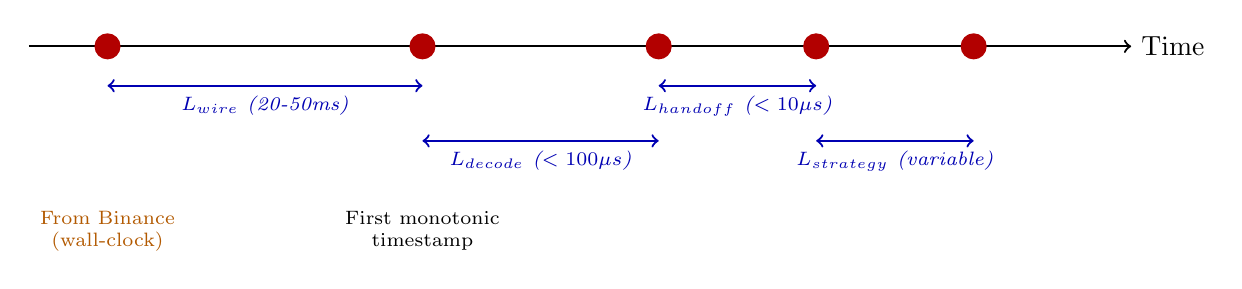
\begin{tikzpicture}[
    point/.style={circle, fill=red!70!black, minimum size=0.15cm},
    label/.style={font=\scriptsize},
    latency/.style={font=\scriptsize\itshape, text=blue!70!black}
]

% Timeline
\draw[thick, ->] (0,0) -- (14,0) node[right] {Time};

% Points
\node[point, label=above:$T_{exchange}$] (tex) at (1,0) {};
\node[point, label=above:$T_{recv}$] (trec) at (5,0) {};
\node[point, label=above:$T_{decoded}$] (tdec) at (8,0) {};
\node[point, label=above:$T_{handoff}$] (than) at (10,0) {};
\node[point, label=above:$T_{strategy}$] (tstr) at (12,0) {};

% Latency spans
\draw[<->, thick, blue!70!black] (1,-0.5) -- (5,-0.5) node[midway, below, latency] {$L_{wire}$ (20-50ms)};
\draw[<->, thick, blue!70!black] (5,-1.2) -- (8,-1.2) node[midway, below, latency] {$L_{decode}$ ($<100\mu s$)};
\draw[<->, thick, blue!70!black] (8,-0.5) -- (10,-0.5) node[midway, below, latency] {$L_{handoff}$ ($<10\mu s$)};
\draw[<->, thick, blue!70!black] (10,-1.2) -- (12,-1.2) node[midway, below, latency] {$L_{strategy}$ (variable)};

% Notes
\node[below=1.8cm of trec, font=\scriptsize, align=center] {First monotonic\\timestamp};
\node[below=1.8cm of tex, font=\scriptsize, align=center, text=orange!70!black] {From Binance\\(wall-clock)};

\end{tikzpicture}
\caption{Per-Message Latency Breakdown}
\end{figure}

\subsection{Histogram Implementation}

The harness uses logarithmic buckets for percentile calculation:

\begin{lstlisting}[style=rustcode, caption=Histogram Bucket Bounds]
let bucket_bounds_ns: Vec<u64> = vec![
    1_000,       // 1 us
    2_000,       // 2 us
    5_000,       // 5 us
    10_000,      // 10 us
    // ... logarithmic progression
    1_000_000_000,  // 1 s
    10_000_000_000, // 10 s
    u64::MAX,
];
\end{lstlisting}

\subsection{Jitter Calculation (RFC 3550)}

\begin{equation}
J_i = J_{i-1} + \frac{|D_{i-1,i}| - J_{i-1}}{16}
\end{equation}

where $D_{i-1,i}$ is the difference between consecutive latency samples.

\subsection{CSV Export Schema}

\begin{table}[H]
\centering
\footnotesize
\begin{tabular}{lll}
\toprule
\textbf{Column} & \textbf{Type} & \textbf{Description} \\
\midrule
\texttt{sample\_id} & u64 & Unique monotonically increasing ID \\
\texttt{symbol} & string & Trading pair (e.g., ``BTCUSDT'') \\
\texttt{wall\_clock\_iso} & string & ISO 8601 timestamp at recv() \\
\texttt{exchange\_ts\_ms} & i64 & Binance exchange timestamp \\
\texttt{mono\_recv\_ns} & u64 & Monotonic ns at recv() \\
\texttt{mono\_decoded\_ns} & u64 & Monotonic ns after decode \\
\texttt{wire\_latency\_ns} & i64 & Estimated one-way (requires NTP) \\
\texttt{decode\_latency\_ns} & u64 & JSON parse time (monotonic) \\
\texttt{total\_internal\_latency\_ns} & u64 & recv $\rightarrow$ strategy \\
\bottomrule
\end{tabular}
\caption{Message Latency CSV Schema}
\end{table}

%==============================================================================
\section{Expected Latency Ranges}
%==============================================================================

\subsection{AWS EU-West-1 $\rightarrow$ Binance}

\begin{table}[H]
\centering
\begin{tabular}{lcccc}
\toprule
\textbf{Component} & \textbf{P50} & \textbf{P95} & \textbf{P99} & \textbf{P99.9} \\
\midrule
DNS resolution & $<1$ ms & 2 ms & 5 ms & 10 ms \\
TCP connect & 15-25 ms & 30 ms & 50 ms & 100 ms \\
TLS handshake & 30-50 ms & 60 ms & 80 ms & 150 ms \\
WS upgrade & 10-20 ms & 25 ms & 35 ms & 50 ms \\
\midrule
\textbf{Total Connect} & \textbf{60-100 ms} & 120 ms & 170 ms & 300 ms \\
\midrule
Wire (one-way)* & 8-15 ms & 20 ms & 30 ms & 50 ms \\
Decode & 10-30 $\mu$s & 50 $\mu$s & 80 $\mu$s & 150 $\mu$s \\
Handoff & 1-5 $\mu$s & 10 $\mu$s & 20 $\mu$s & 50 $\mu$s \\
Strategy queue & 5-20 $\mu$s & 50 $\mu$s & 100 $\mu$s & 500 $\mu$s \\
\midrule
\textbf{Total Internal} & \textbf{20-60 $\mu$s} & 120 $\mu$s & 200 $\mu$s & 700 $\mu$s \\
\bottomrule
\end{tabular}
\caption{Expected Latency Ranges (*Wire latency requires NTP sync, accuracy $\pm 1-5$ ms)}
\end{table}

%==============================================================================
\section{Edge Receiver Architecture (Experimental)}
%==============================================================================

\subsection{Overview}

For ultra-low latency requirements, the edge receiver architecture places a co-located server near Binance infrastructure that forwards market data via UDP multicast.

\begin{figure}[H]
\centering
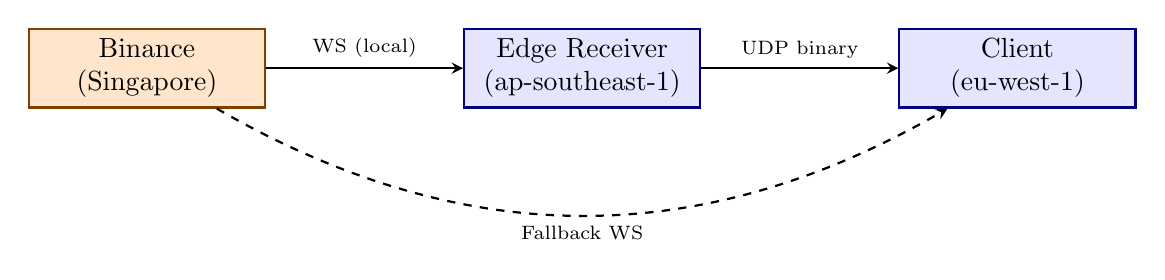
\begin{tikzpicture}[
    node distance=2cm,
    box/.style={rectangle, draw=blue!50!black, fill=blue!10, thick, minimum height=1cm, minimum width=3cm, align=center},
    arrow/.style={->, thick, >=stealth}
]

\node[box, fill=orange!20, draw=orange!50!black] (binance) {Binance\\(Singapore)};
\node[box, right=2.5cm of binance] (edge) {Edge Receiver\\(ap-southeast-1)};
\node[box, right=2.5cm of edge] (client) {Client\\(eu-west-1)};

\draw[arrow] (binance) -- node[above, font=\scriptsize] {WS (local)} (edge);
\draw[arrow] (edge) -- node[above, font=\scriptsize] {UDP binary} (client);
\draw[arrow, dashed, bend right=30] (binance) to node[below, font=\scriptsize] {Fallback WS} (client);

\end{tikzpicture}
\caption{Edge Receiver Deployment}
\end{figure}

\subsection{Wire Protocol}

\begin{lstlisting}[style=rustcode, caption=EdgeTick Wire Format (32 bytes)]
pub struct EdgeTick {
    pub symbol: u8,          // Symbol ID (0=BTC, 1=ETH, etc.)
    pub seq: u64,            // Sequence number
    pub exchange_ts_us: u64, // Exchange timestamp (microseconds)
    pub recv_ts_us: u64,     // Edge receive timestamp
    pub bid: u32,            // Bid price (fixed-point)
    pub ask: u32,            // Ask price (fixed-point)
    pub bid_qty: u16,        // Bid quantity (scaled)
    pub ask_qty: u16,        // Ask quantity (scaled)
    pub flags: u8,           // Heartbeat, compression flags
    pub checksum: u8,        // CRC8 checksum
}
\end{lstlisting}

\subsection{Loss Detection and Reordering}

\begin{itemize}
    \item \textbf{Reorder buffer}: 16 packets, 5 ms timeout
    \item \textbf{Gap detection}: Sequence tracking with statistics
    \item \textbf{QUIC fallback}: Activates when loss ratio $> 1\%$ over 60s
    \item \textbf{Heartbeat timeout}: 500 ms triggers fallback
\end{itemize}

%==============================================================================
\section{Configuration Reference}
%==============================================================================

\subsection{Environment Variables}

\begin{table}[H]
\centering
\footnotesize
\begin{tabular}{lp{3cm}p{5cm}}
\toprule
\textbf{Variable} & \textbf{Default} & \textbf{Description} \\
\midrule
\texttt{BINANCE\_ENABLED} & \texttt{true} & Enable Binance price feed \\
\texttt{BINANCE\_BACKOFF\_BASE\_MS} & 100 & Initial reconnect delay \\
\texttt{BINANCE\_BACKOFF\_MAX\_MS} & 30000 & Maximum reconnect delay \\
\texttt{BINANCE\_CONNECT\_TIMEOUT\_MS} & 10000 & Connection timeout \\
\texttt{BINANCE\_PING\_INTERVAL\_MS} & 30000 & WebSocket ping interval \\
\texttt{BINANCE\_STALE\_DATA\_TIMEOUT\_MS} & 5000 & Max time without data \\
\texttt{BINANCE\_HFT\_PIN\_CORE} & -- & CPU core for ingest thread \\
\texttt{BINANCE\_HFT\_EWMA\_LAMBDA} & 0.97 & Volatility EWMA decay \\
\bottomrule
\end{tabular}
\caption{Binance Feed Environment Variables}
\end{table}

%==============================================================================
\section{Appendix: Benchmark Results}
%==============================================================================

\subsection{Microbenchmark Targets}

\begin{table}[H]
\centering
\begin{tabular}{lccl}
\toprule
\textbf{Benchmark} & \textbf{P50} & \textbf{P99} & \textbf{Target} \\
\midrule
SeqLock write & 20 ns & 50 ns & $< 100$ ns \\
SeqLock read (uncontended) & 15 ns & 30 ns & $< 50$ ns \\
Symbol update (with EWMA) & 100 ns & 200 ns & $< 500$ ns \\
JSON parse (manual) & 150 ns & 300 ns & $< 500$ ns \\
JSON parse (serde) & 800 ns & 2000 ns & baseline \\
Full message processing & 300 ns & 600 ns & $< 1 \mu s$ \\
\bottomrule
\end{tabular}
\caption{Expected Microbenchmark Results (release mode, modern x86)}
\end{table}

%==============================================================================
\section{Conclusion}
%==============================================================================

The Binance price feed architecture provides a layered approach to market data ingestion, allowing selection of the appropriate trade-off between complexity and latency:

\begin{enumerate}
    \item For most use cases, \texttt{BinancePriceFeed} with \texttt{barter-data} provides excellent reliability with reasonable latency
    \item For latency-sensitive applications, \texttt{BinanceBookTickerFeed} with SIMD parsing offers sub-100$\mu$s decode times
    \item For HFT workloads, \texttt{BinanceHftIngest} with SeqLock provides zero-allocation reads at $\approx 50$ ns
    \item \texttt{HardenedBinanceIngest} wraps any backend with production-grade fault tolerance
    \item The edge receiver architecture provides a path to sub-millisecond latency when co-location is available
\end{enumerate}

The comprehensive latency harness enables continuous monitoring and optimization of all pipeline stages.

\end{document}
